%\title{Two column article template by M.A.}

\documentclass[11pt, twocolumn]{article}

\usepackage{authblk}

\makeatletter
\renewcommand{\maketitle}{\bgroup\setlength{\parindent}{0pt}
\begin{flushleft}
  \textbf{\@title}

  \@author
\end{flushleft}\egroup
}
\makeatother


%  Set the title and author.
\title{\Huge Mapping governance networks through hyperlink analysis: What do we really measure?  \vspace{0.5cm}}
\author{\Large Mario Angst \normalsize \hspace{0.5cm} Eawag aquatic research, University of Berne}


\date{\today}

\usepackage[showframe=false, margin=.75in]{geometry}

\usepackage{abstract}
\renewcommand{\abstractname}{}    % clear the title
\renewcommand{\absnamepos}{empty} % originally center

\usepackage{lipsum}

\usepackage{afterpage}

\renewenvironment{abstract}
 {\small
  \begin{center}
  \bfseries \abstractname\vspace{-.5em}\vspace{0pt}
  \end{center}
  \list{}{%
    \setlength{\leftmargin}{10mm}% <---------- Change margin here
    \setlength{\rightmargin}{\leftmargin}%
  }%
  \item\relax}
 {\endlist}

\usepackage[utf8]{inputenc}

%\usepackage{graphicx}
\usepackage{wrapfig}
\usepackage[lofdepth,lotdepth]{subfig}
\usepackage{booktabs}

\usepackage{rotating}

\usepackage{caption}
%\usepackage{subcaption}

%\usepackage[ngerman]{babel}

\usepackage{csquotes}

\usepackage{todonotes}

\usepackage{stfloats}

\usepackage[T1]{fontenc}
\usepackage{textcomp}
\usepackage{times}

\usepackage{framed} %um Boxen zu machen

%\usepackage[citestyle=authoryear,
%			bibstyle=authoryear,
%			language=auto,
%			url=false,
%			backend=bibtex,
%			doi=false,
%			isbn=false]{biblatex}

\usepackage[hyperref=true, backend=biber, sorting=none,backref=true]{biblatex}
%\usepackage{biblatex}
%\usepackage[numbers,sort&compress]{natbib}

	\renewbibmacro*{volume+number+eid}{%
  \printfield{volume}%
%  \setunit*{\adddot}% DELETED
  \setunit*{\addnbspace}% NEW (optional); there's also \addnbthinspace
  \printfield{number}%
  \setunit{\addcomma\space}%
  \printfield{eid}}
\DeclareFieldFormat[article]{number}{\mkbibparens{#1}}
\addbibresource{Mendeley.bib}

\usepackage{setspace}
\onehalfspacing

\setlength{\columnsep}{0.8cm}

\setlength{\parskip}{0em}

\usepackage{color}
\definecolor{black}{gray}{0} % 10% gray

\usepackage[colorlinks=true,linkcolor=black,citecolor=black]{hyperref}

\usepackage{tabularx}
\newcolumntype{b}{X}
\newcolumntype{s}{>{\hsize=.5\hsize}X}

\usepackage{ntheorem}
\newtheorem*{TRQ}{Research Question}

\newtheorem{Hyp}{Hypothesis} 


\begin{document}

\twocolumn[
\begin{@twocolumnfalse}
\maketitle
\begin{abstract}
\textit{\lipsum[1]
\bigskip}
\end{abstract}
\end{@twocolumnfalse}
]

%First we are citing \textcite{Authors14}.
First we are citing ~\parencite{Alpher02}.

\lipsum[1]

\begin{Hyp}
A hypothesis is likely to be false if it is longer than this line
\label{hyp:nd_conflictivity}
\end{Hyp}

\lipsum[1]

\begin{table}[ht]
\centering
\begin{tabular}{rrrrrr}
  \toprule[1.5pt]
  text & text & text & text & text & text  \\
  \midrule[0.8pt]
  1 &  84 &  46 &   4 &   3 &   5 \\
    2 &  67 &  24 &   5 &   1 &   5 \\
    3 &  54 &  26 &   4 &   2 &   5 \\
    4 &  44 &  16 &   5 &   2 &   5 \\
    5 &  53 &  21 &   6 &   2 &   5 \\
   \bottomrule[1.5pt]
\end{tabular}
\caption{An example single column table}
\label{tab:example}
\end{table}

\lipsum[1]

\begin{figure*}[ht!]
\centering
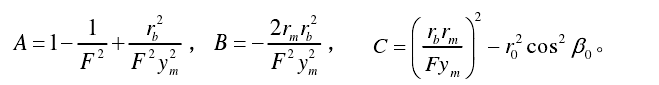
\includegraphics[width=1\textwidth]{picture/equation.png}
\caption{A two column figure (indicate with figure*)}
\label{fig:example}
\end{figure*}

\lipsum[1]

\printbibliography

\clearpage
\appendix
\renewcommand\thefigure{A\arabic{figure}}
\setcounter{figure}{0}

\section*{Appendix}

Appendix content

\subsection*{Appendix A}
\lipsum[2]

\end{document}